\chapter{Реализация архитектур}

\section{Подготовка данных}

\subsection{Описание}

Исходные данные представляют собой таблицу в формате Microsoft Excel, где каждой строке соответствует определенный километр пути,
а столбцу~--- определенный параметр состояния (например, дефект). Далее будем называть строки этой таблицы 
\textit{объектами}, а столбцы~--- \textit{признаками}.

Строго говоря, признак~--- результат измерения некоторой характеристики объекта, т.\,е. отображение
\begin{equation*}\label{def_feature}
		f: X \rightarrow D_f,
\end{equation*}
где $ X $~--- множество объектов, $ D_f $~--- множество допустимых значений признака.
В зависимости от вида множества $ D_f $ признаки делятся на~следующие типы:
\begin{itemize}[noitemsep, wide]
	\item бинарный: $ D_{f}=\{0,1\} $,
	\item номинальный: $ D_f $ — конечное множество,
	\item порядковый: $ D_f $ — конечное упорядоченное множество,
	\item количественный: $ D_f $ — множество действительных чисел.
\end{itemize}

Перед тем как строить признаковое описание объектов, необходимо проанализировать, что
из себя представляют исходные признаки и какие связи есть между ними:
\begin{table}[!h]\centering
	\vspace{-2mm}
	\caption{Типы признаков}\medskip
	
	\begin{tabular}{|m{5cm}|>{\centering}m{3cm}|m{5cm}|}
		\hline
		
		\bf Тип & \bf Количество & \bf Пример \\ \hline
		
		Бинарный &  23 & Восемь и более\newline просадок на отрезке длиной 100~м \\ \hline 
		
		Номинальный & 91 & Количество просадок 1 степени \\ \hline
		
		Порядковый & 6 & Код дороги, год и \newline месяц измерения \\ \hline 
	
		Количественный признак & 20 & Дистанция пути \\ \hline
		
		Принимает единственное значение & 4 & Отступления\newline с~просадкой \\ \hline 
\end{tabular}
	\vspace{-3mm}
\end{table}

Б\'{о}льшая часть признаков номинальна. Эти признаки\linebreak показывают
ту или иную степень отклонения железнодорожного полотна от~нормы. В равной степени встречаются бинарные и~количественные
признаки. Меньше всего порядковых признаков и~признаков, принимающих единственное значение.

Итоговые признаки, которые подаются на вход модели, необязательно 
должны состоять только из исходных сырых данных.
В качестве итоговых признаков могут быть взяты:
\begin{itemize}[wide, noitemsep, topsep=-\parskip]
	\item признаки, придуманные исходя из анализа основных свойств данных и
	нахождения в них общих закономерностей \cite{tensorflow2015-whitepaper};
	
	\item признаки, полученные из исходных данных по некоторому правилу (косвенные признаки);
	
	\item смешанные признаки.
\end{itemize}

\medskip
Выбор итоговых признаков для конкретных моделей описан в дальнейшем в соответствующих главах.



\subsection{Анализ данных}

Визуализируем исходные данные.
Для начала узнаем, как меняется общее число отказов с течением времени (см. рис.~\ref{breaks_num}).
Можно заметить, что в летние месяцы в среднем количество отказов больше, чем в зимний период.
Отсюда можно сделать следующие предположения:
\begin{itemize}
	\item летом движение более интенсивное, т.\,е. нагрузка выше;
	
	\item летом рельсы под воздействием тепла больше склонны к~деформации, 
	следовательно, чаще выходят из строя;
	
	\item летом проводится больше измерений различных путей, и чем больше 
	измерений делается, тем больше отказов находят.
\end{itemize}

Попробуем проверить последнее предположение. Для этого построим график с общим 
числом проверок сгруппировав их по дням (см. рис~\ref{check_num}). Видно,
что <<горбы>> на соответствующих графиках практически совпадают.
Следовательно, что есть некоторая зависимость между числом проверок и количеством
отказов, то есть чем больше проверок производится, тем больше отказов находят.


После большого количества проверок, а~следовательно и~ремонтов, 
количество выходов из~строя железнодорожных путей резко падает. 
Поэтому было принято решение к~исходным признакам добавить признак
 <<количество проверок в~прошлом месяце>> на~данном участке пути.
 
Из~анализа данных об~отказах железнодорожных путей видно, что не~все отказы были 
правильно зарегистрированы. Отсутствует информация о~том, где именно 
произошел отказ. Значит, не~представляется возможным верно назначить данные об~отказе
определенному объекту железнодородного пути. Для~таких объектов в~стобце
TARGET указано значение~0 (объект без~опасного отказа) несмотря на~то, что отказ был.
 
Таким образом, данные оказываются зашумленными. Это приводит к тому, что модель изначально
обучается на некорректном наборе данных. Процент неверных отказов составляет порядка 17\,\%, что 
делает невозможным получение высокой точности предсказания потенциально опасных отказов.

При~резком улучшении состояния километра данное событие классифицировалось 
как~ремонтные работы и~часть наблюдений удалялась, чтобы~в дальнейшем не~<<запутывать>> модель во~время обучения.
База данных по~проводимым ремонтам железнодорожных путей находится в~запущенном состоянии, содержит 
слишком много пропусков и~ошибок, поэтому использовать ее~непосредственно не~представляется возможным.

\begin{landscape}
	\begin{figure}[h]
		\centering
		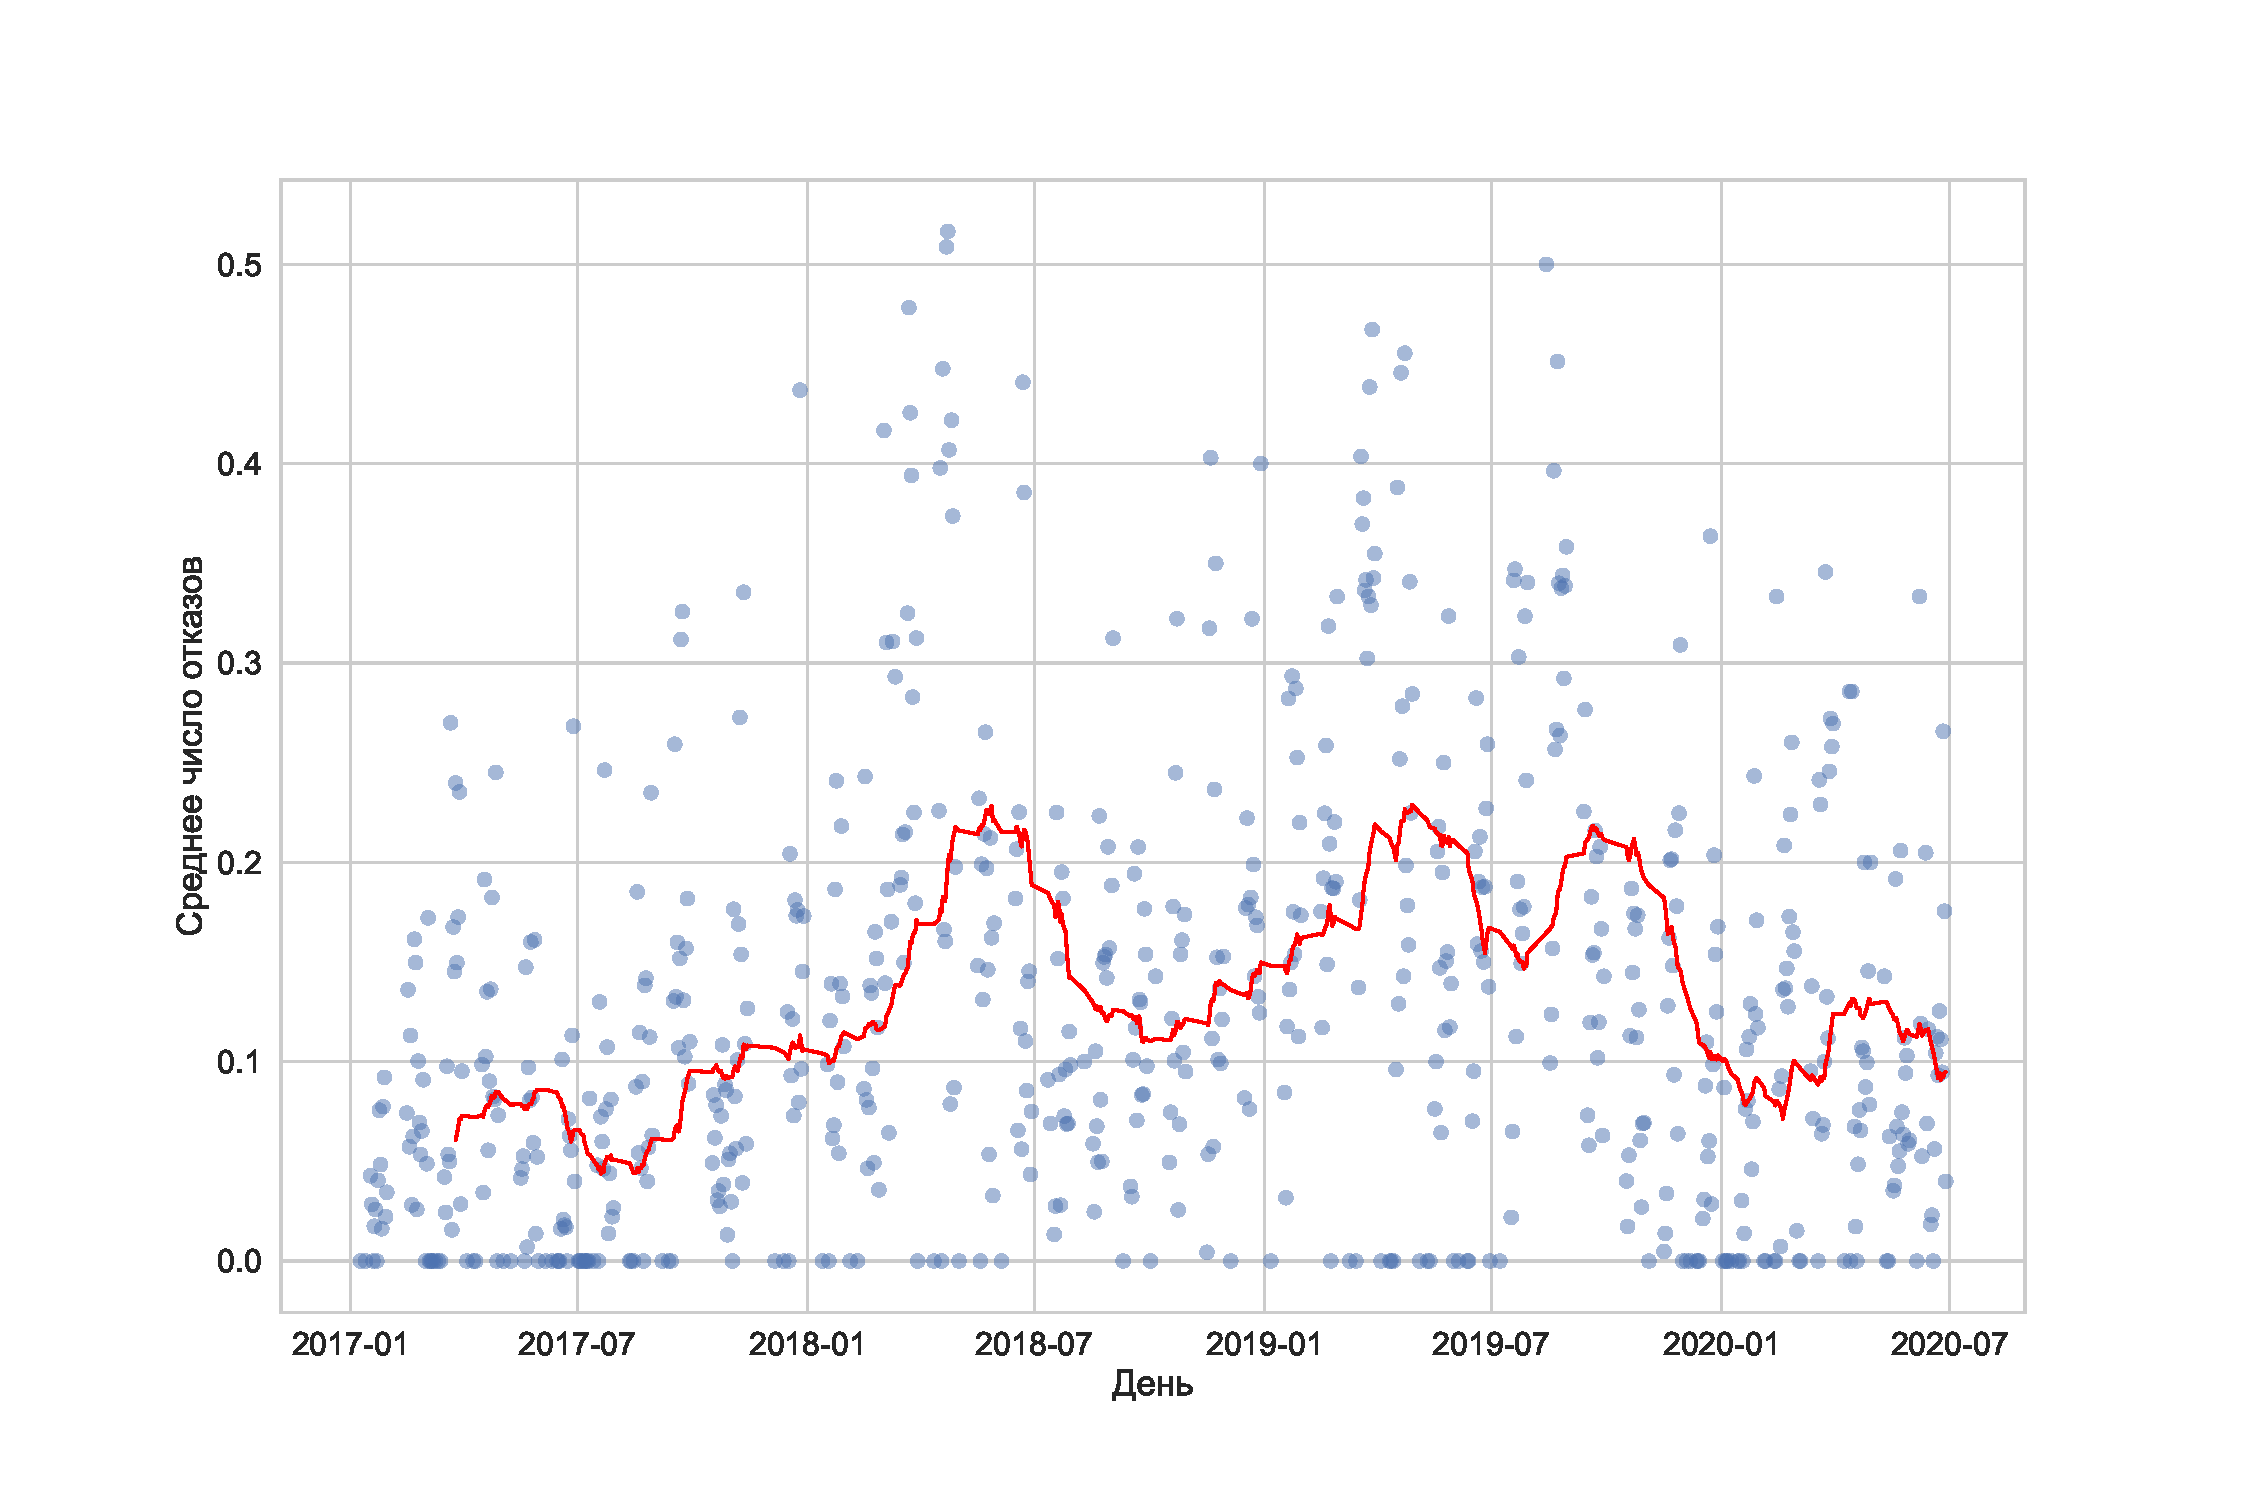
\includegraphics[height=0.9\textwidth, clip, trim={0 1cm 0 3cm}]{pics/breaks_num}
		\caption{Количество отказов от времени}
		\label{breaks_num}
	\end{figure}
\end{landscape}
\begin{landscape}
	\begin{figure}[h]
		\centering
		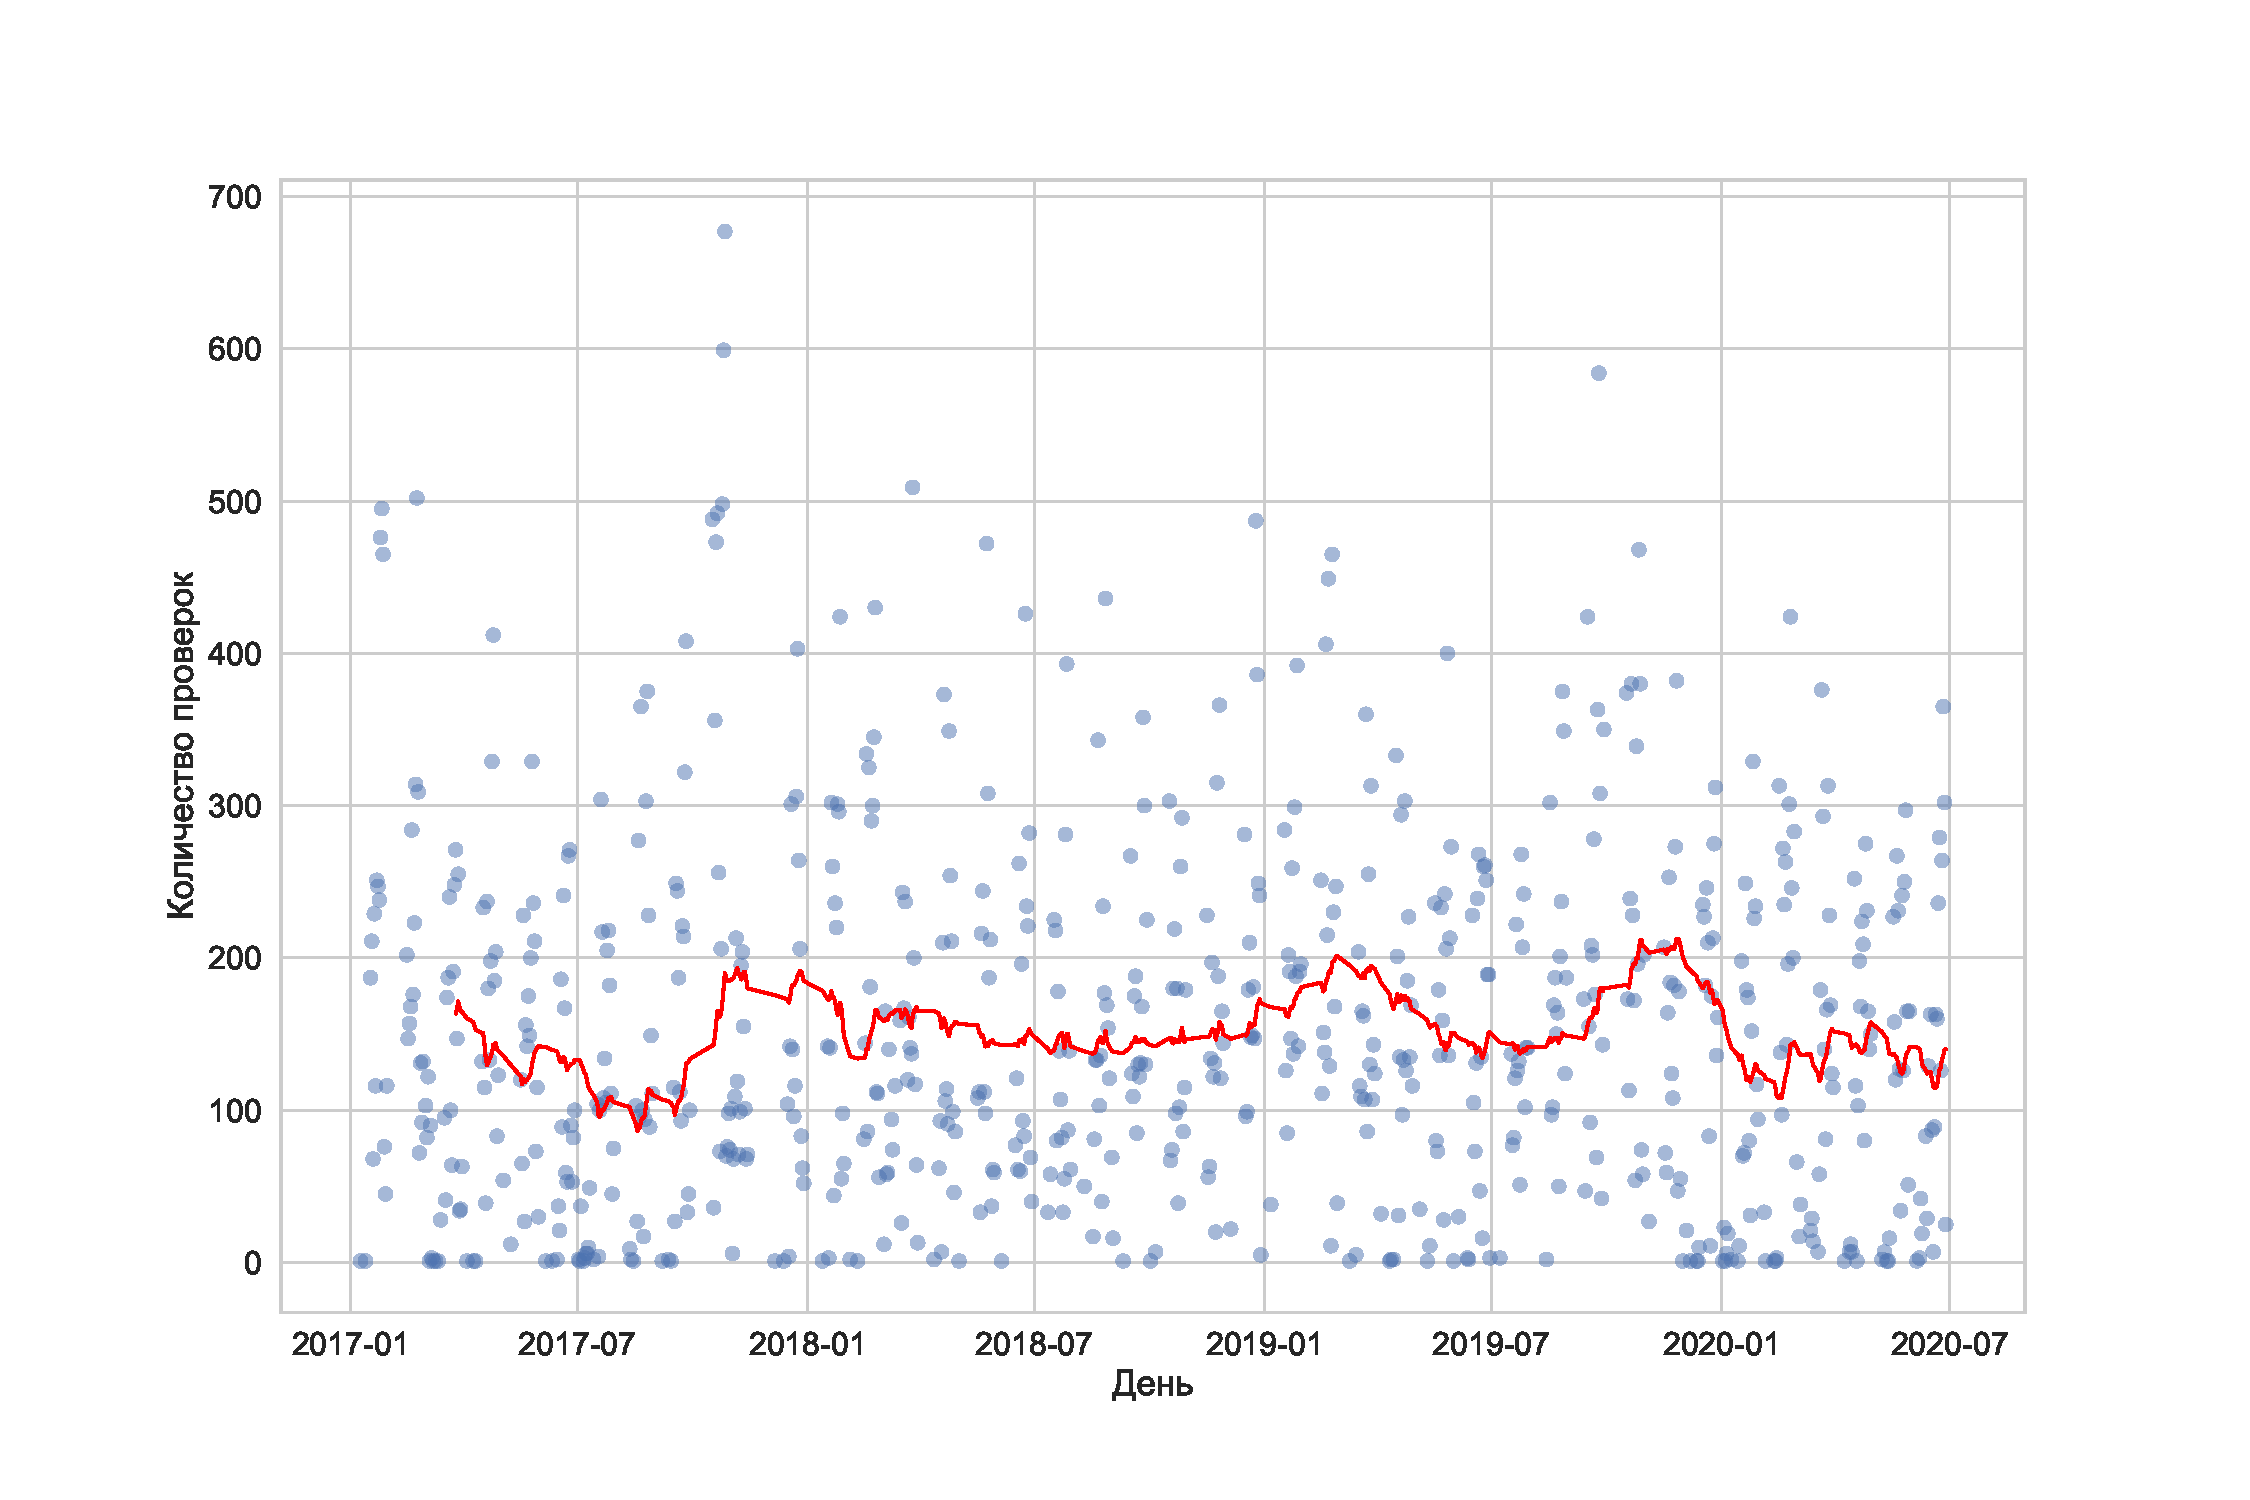
\includegraphics[height=0.9\textwidth, clip, trim={0 1cm 0 3cm}]{pics/check_num}
		\caption{Количество проверок от времени}
		\label{check_num}
	\end{figure}
\end{landscape}

\subsection{Разбиение данных} %  на обучающую, валидационную и тестовую выборки 


Прежде всего для обеспечения корректного обучения моделей необходимо разбить данные
на обучающую, валидационную и тестовую выборки. 

На обучающей выборке модель будет подбирать
нужные параметры сети для минимизации ошибки, на валидационной выборке будут настраиваться гиперпараметры модели
а~на~тестовой выборке будет анализироваться итоговый результат.\linebreak
Ниже приведена таблица с данными по каждой из выборок:
\begin{table}[!h]\label{split_table}\centering
	\caption{Разбиение данных}\medskip
	
	\begin{tabular}{|l|c|}
		\hline
		
		Суммарный объем выборки           & 107597                  \\\hline
		
		Объем обучающей выборки   & 74077                    \\\hline
		
		Объем валидационной выборки    & 17889                                 \\\hline
		
		Объем тестовой выборки    & 15631      \\ \hline
		
		Обучающая выборка                     & январь 2017 -- декабрь 2019     \\\hline
		
		Валидационная выборка                     & январь 2017 -- декабрь 2019     \\\hline
		
		Тестовая выборка                          & январь 2020 -- июнь 2020   \\\hline
		
		Количество признаков                  & 144                         \\\hline
		
	\end{tabular}
\end{table}

На выходе классификатора модели предиктивного анализа получается не 
строгое значение класса, а уверенность в~<<положительном>> результате, 
которая может принимать значения от~0 до~1. Для каждого объекта пути 
классификатор рассчитывает вероятность того, что объект принадлежит к~положительному классу.
Прогноз возникновения опасного отказа строится для~следующего месяца.

\subsection{Выбор порога принятия решения}

Для принятия окончательного решения необходимо задать порог для вероятности~--- threshold. 
Если вероятность меньше этого порога, то объект пути относится к отрицательному 
классу и ему присваивается метка 0 (объект без опасного отказа). 
Если вероятность больше заданного значения threshold, объекту присваивается 
метка 1 (объект с потенциальным опасным отказом).

Выбор порога threshold строится исходя из следующих положений:

\begin{enumerate}[wide]
	\item Порог threshold равен 0,5, если количество 0 и 1 в~поле кодировки целевого 
	признака встречаются одинаково часто и~ошибки в данных имеют симметричное распределение.
	
	\item Если важнее правильно предсказать опасные отказы, то~порог должен быть снижен. 
	Если важнее не допустить появление объектов пути, которые ошибочно будут 
	классифицированы как 1, то порог должен быть увеличен.
\end{enumerate}



\section{Построение моделей}
\subsection{Обучение}

Настоящая работа предполагает работу с больш\'{и}ми объемами данных, 
которые требуют соответствующих затрат вычислительных ресурсов. 

В силу того, что нет возможности загрузить сразу все данные в обработку,
их делят на части меньшего размера, 
загружают их по очереди и обновляют веса нейронной сети в конце каждого шага, 
подстраивая их под данные.

\clearpage
Далее используются следующие понятия:
\begin{itemize}[wide]
	\item \textbf{epoch}~--- эпоха: количество прохождений всего набора данных через нейронную 
	сеть в~обоих направлениях;
	
	\item \textbf{batch}~--- батч: часть набора данных (обычно значительно меньше, чем весь набор данных);
	
	\item \textbf{batch size}~--- общее число тренировочных объектов, 
	представленных в одном батче;
	
	\item \textbf{iteration}~--- число батчей, необходимых для~завершения одной эпохи.
\end{itemize}

\subsection{Измерение результатов}
Естественным, простым и распространённым функционалом качества является точность (англ. Accuracy)~---
доля объектов, на которых модель выдала правильные ответы. Недостаток такого функционала 
очевиден: он плох в случае дисбаланса классов, когда представителей одного из класса существенно 
больше, чем другого. В этом случае, с точки зрения точности, выгодно почти всегда выдавать 
метку самого популярного класса. 

Поэтому для измерения качества модели было решено использовать следущую метрику, аналогичную 
точности, в случае дисбаланса классов: 
\[
\mathtt{balanced\ accuracy = \frac{TPR+TNR}{2}},
\]
где $ \mathtt{TPR} $~--- процент правильно классифицированных объектов положительно класса,
$ \mathtt{TNR} $~--- процент правильно классифицированных объектов негативного класса.

Рассмотрим матрицу несоответствий (англ. confusion matrix) на рис.~\ref{conf_mtrx}.

\begin{figure}[h]
	\centering
	\hspace{-3cm}
		\noindent
	\renewcommand\arraystretch{1.5}
	\setlength\tabcolsep{0pt}
	\begin{tabular}{m{1.7cm}r @{\hspace{0.7em}}c @{\hspace{0.7em}}c }
		\multirow{10}{*}{\rotatebox{90}{\parbox{2.5cm}{\centering \bfseries Правильные \\ метки  \hspace{1cm}}}} 
		& \bfseries Ответ 
		& \multicolumn{2}{c}{\bfseries модели\medskip}\\ 
		& \MyBox{True}{Positive} & \MyBox{False}{Negative}\\[2.4em]
		& \MyBox{False}{Positive} & \MyBox{True}{Negative}\\
		
	\end{tabular}

	\caption{Матрица несоответствий \cite{conf_mtrx}}
	\label{conf_mtrx}
\end{figure}

Объекты, которые модель относит к положительному классу (метка 1), называются положительными (Positive), 
те из них, которые на самом деле принадлежат к этому классу~--- истинно положительными (True Positive), 
остальные~--- ложно положительными (False Positive). Аналогичная терминология есть для отрицательного (Negative) класса (метка 0). 
Дальше используем естественные сокращения:
\begin{itemize}[noitemsep, wide]
	\item TP = True Positive,
	\item TN = True Negative,
	\item FP = False Positive,
	\item FN = False Negative.
\end{itemize}

В этих терминах исходный функционал качества принимает следующий вид:
\[
		\mathtt{balanced\ accuracy = \frac{TPR+TNR}{2} = \frac{1}{2}\left(\frac{TP}{TP+FN} + \frac{TN}{TN+FP}\right)}.
\]

Если в бинарной задаче классификации представителей двух классов примерно поровну, 
то $ \mathtt{TP + FN \approx TN + FP}  $, и сбалансированная точность примерно равна точности обычной (Accuracy).

\subsection{Полносвязная нейронная сеть}

\paragraph{Формат входных данных}~\\
Входные данные представляют собой тензор размера \texttt{(batch\_size,~num\_features)}, 
где  \texttt{num\_features}~--- количество признаков в итоговом датасете.

\vspace{-2ex}
\paragraph{Предложенная архитектура}~\\
Данная нейронная сеть состоит из четырех полносвязных слоев и функции активации ReLU \cite{act_func} между ними. 
На выходе сети стоит функция активации Sigmoid, которая переводит множество выходных
значений модели в отрезок $ [0, 1] $, что по смыслу соответствует вероятности наличия положительного класса 1.

\vspace{-2ex}
\paragraph{Используемые гиперпараметры}~\\
Количество эпох: \ \texttt{num\_epoch = 50}\\
Размер батча: \ \texttt{batch\_size = 1024}\\
Количество признаков: \ \texttt{num\_features = 144}\\
Количество нейронов в скрытом слое: \ \texttt{num\_hidden = 50}

\vspace{-2ex}
\paragraph{Результаты}~\\
Оптимальный порог: \ \texttt{best\ threshold = 0.19}\\
При~этом пороге матрица несоответствий имеет следующий вид:

\begin{table}[!h]
	\centering
	\caption{Матрица несоответствий для полносвязной НС}\medskip
	\begin{tabular}{l|l|c|c|c}
\multicolumn{2}{c}{}&\multicolumn{2}{c}{Правильные метки}&\\
\cline{3-4}
\multicolumn{2}{c|}{}&Истина&Ложь&\multicolumn{1}{c}{Всего}\\
\cline{2-4}
\multirow{2}{*}{Предсказания }& Истина & $ 10156 $ & $ 3253 $ & $ 13409$\\
\cline{2-4}
& Ложь & $474$ & $1367$ & $ 1841 $\\
\cline{2-4}
\multicolumn{1}{c}{} & \multicolumn{1}{c}{Всего} & \multicolumn{1}{c}{$10630$} & \multicolumn{1}{c}{$4620$} & \multicolumn{1}{c}{$15250$}\\
\end{tabular}
	\label{FFNN_conf_mtrx}
\end{table}

\noindent
Функционал качества: \ \texttt{balanced\ accuracy = 0.7504}

\subsection{Рекуррентная нейронная сеть}

Для рекуррентной нейронной сети важна предистория наблюдений, поэтому по~сравнению с~предыдущим вариантом необходимо добавить размерность \texttt{history\_size}.

Опишем процедуру формирования предыстории:
\begin{enumerate}[wide]
		\item В исходных данных целевое значение, столбец TARGET, показывает отказ в \textit{следующем} месяце, 
		поэтому	его необходимо сдвинуть на одну позицию вниз. Каждому километру пути соответствует строка признаков, в которой значение TARGET показывает,
		был ли отказ пути с заданными признаками.
		
		\item Отсортировать все данные по~признакам в следующем порядке: КМ (километр), ГОД, МЕСЯЦ, ДЕНЬ. Для
		каждого километра таких наблюдений в среднем около 70.
		
		\item Удалить признаки <<ГОД>> и <<ДЕНЬ>>, поскольку они не несут никакой дополнительной информации.
		Признак <<МЕСЯЦ>> оставлен в качестве некоторого климатического фактора: другие данные, которые можно было~бы использовать в~данном качестве, в~исходных данных отсутствуют.
		
		\item По~наблюдениям для~определенного километра пройтись окном размером \texttt{history\_size}
		с~шагом \texttt{step} (см. рис.~\ref{data_window}).
\end{enumerate}

В~данном формате рекуррентная нейронная готова предсказывать следующее значение 
целевой переменной по~заданному набору измерений.

\begin{figure}[h]
	\centering
	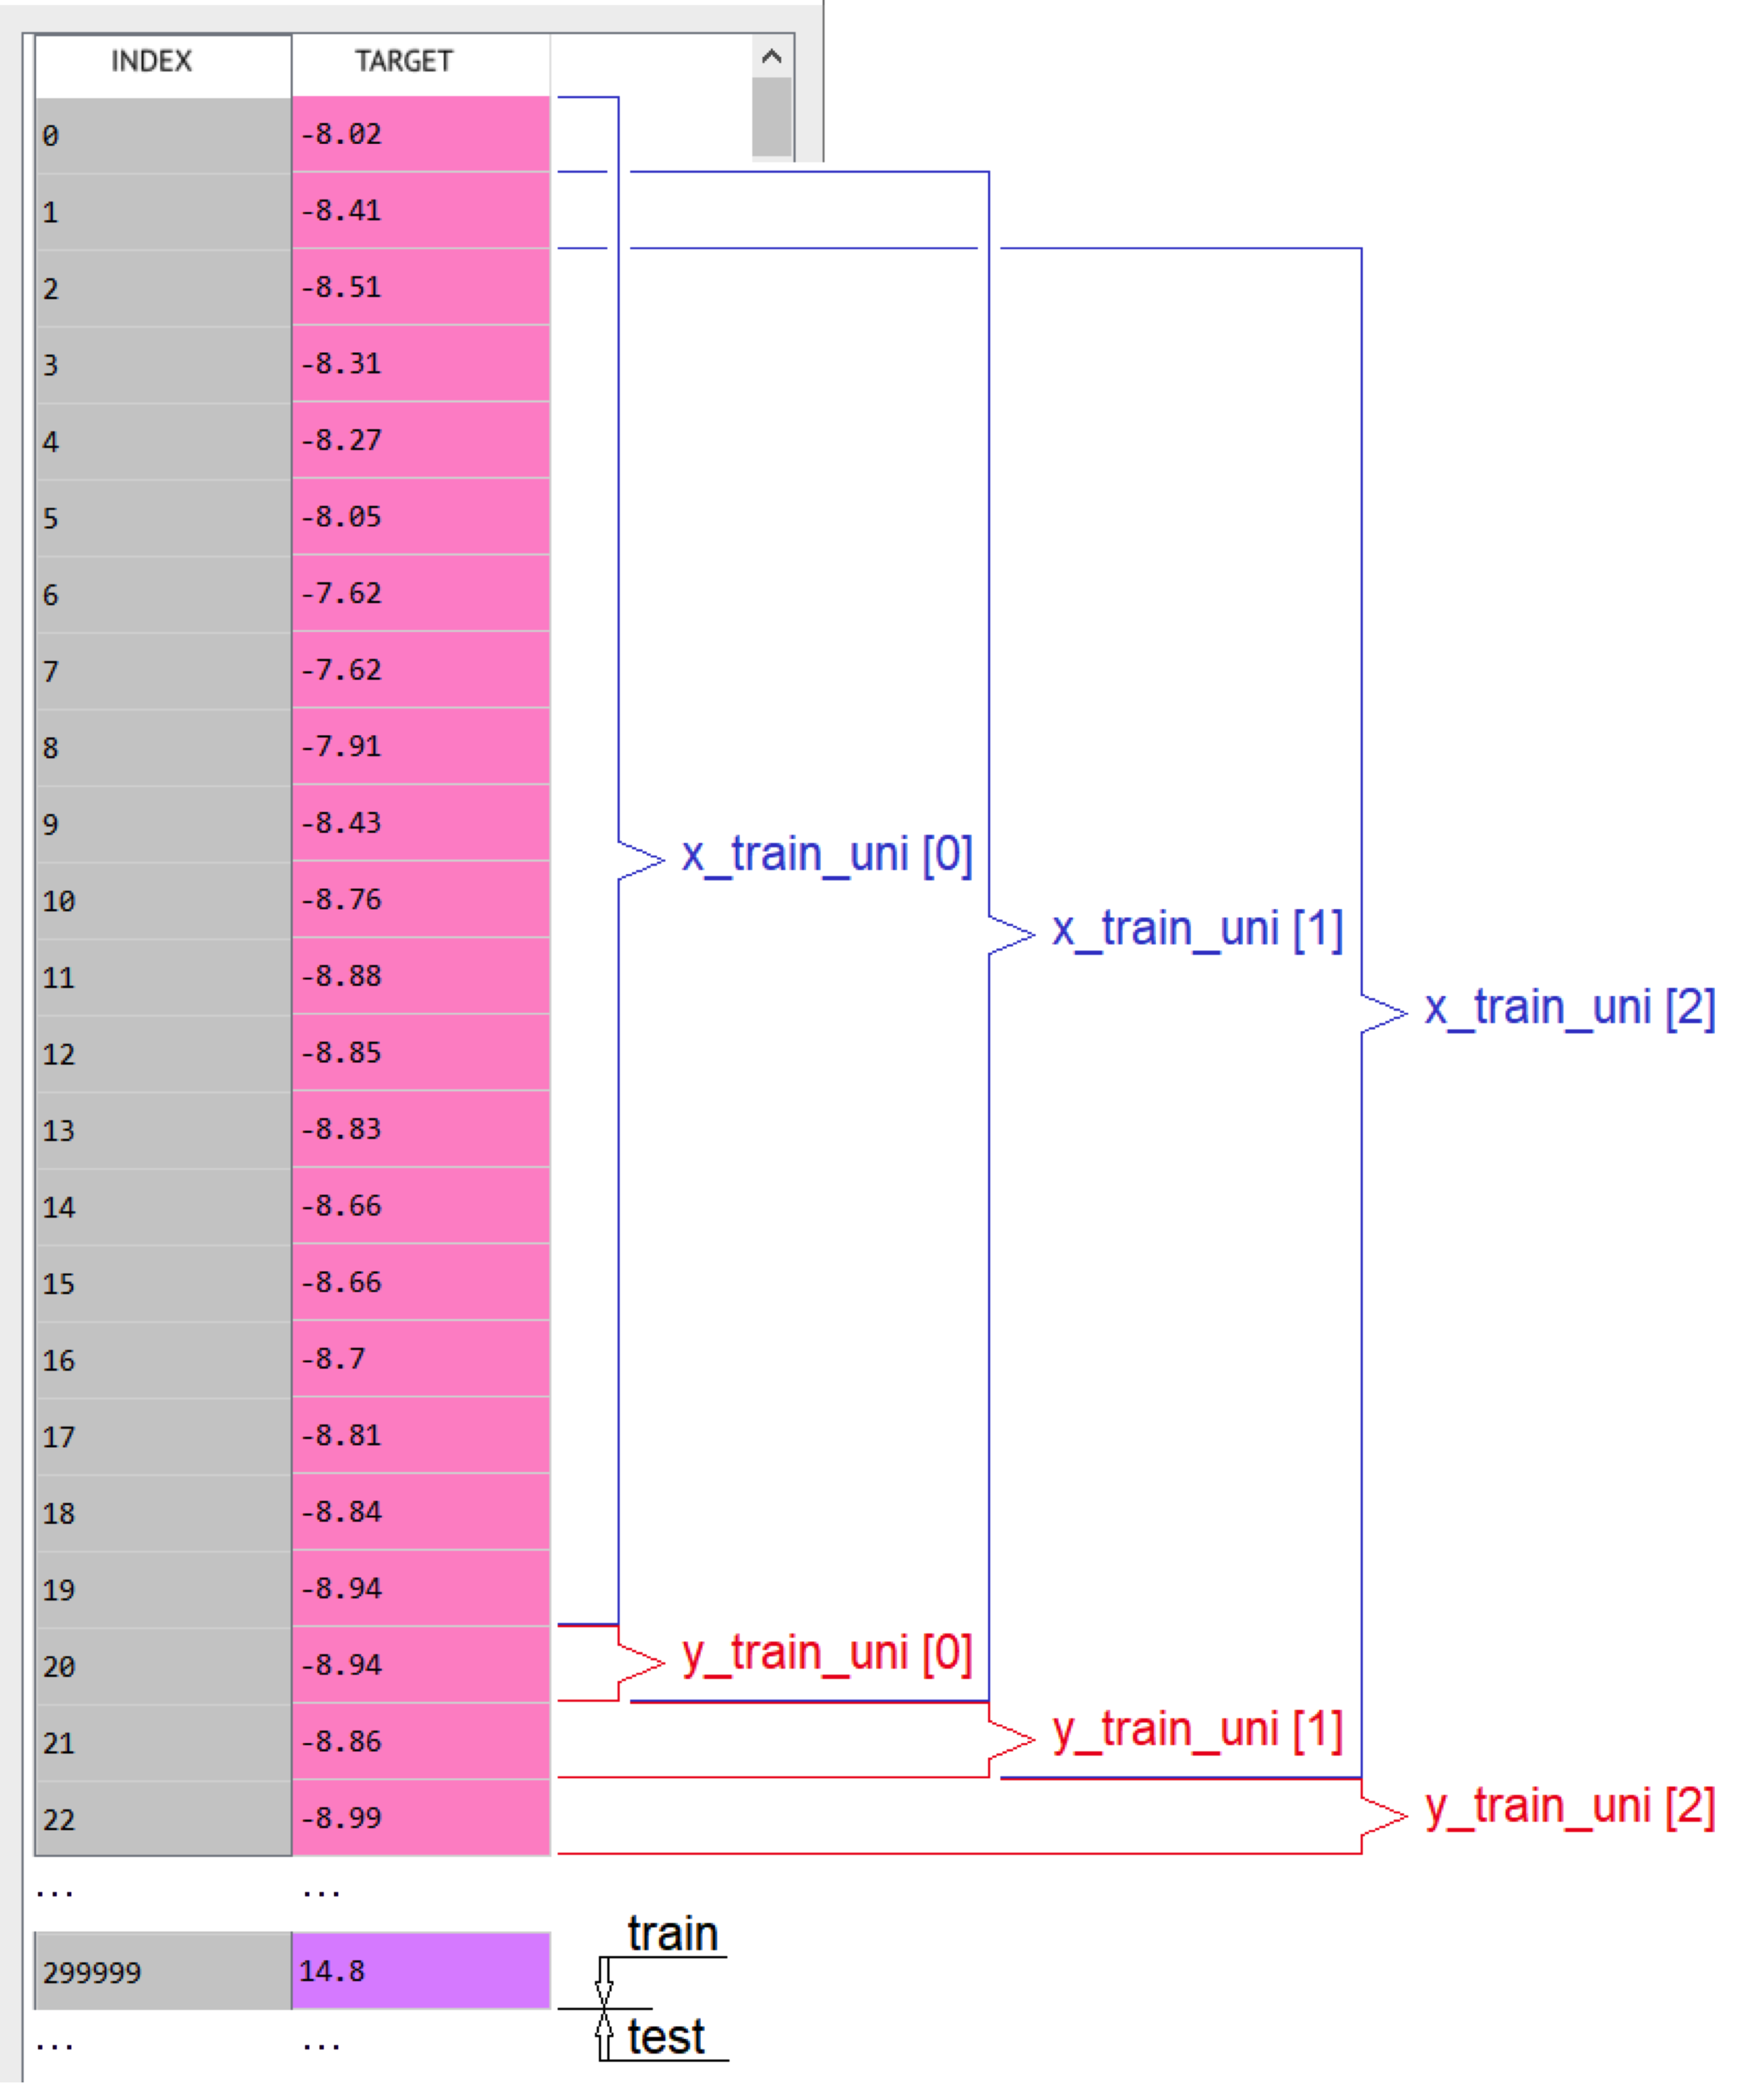
\includegraphics[width=\textwidth, clip, trim={1cm 0 1.2cm 0}]{pics/data_window}
	\caption{Процесс прохода по данным окном}
	\label{data_window}
\end{figure}

\clearpage
Если взять полученные данные и подать без предварительной обработки, качество на выходе будет
сопоставимо с~моделью случайного угадывания. Поэтому далее приведены этапы обработки данных для 
рекуррентной сети, которые помогли существенно повысить качество для обеих рекуррентных моделей RNN и GRU:
\begin{enumerate}[wide]
	\item Перемешивание данных на обучающей выборке. Чтобы модель была более устойчива по~входным
	данным, необходимо в~процессе обучения подавать данные не~в~хронологическом порядке, а~в~случайном.
	
	\item Нормировка данных. Все данные приводятся к нормальному виду путем вычитания среднего значения
	и деления на дисперсию. Это обычная практика, которая часто заметно улучшает итоговое качество моделей
	машинного обучения.
	
	\item Уменьшение размерности пространства признаков с~помощью метода главных компонент 
	(PCA). Количество признаков в итоговом наборе данных задается
	параметром \texttt{num\_features}.
	
	\item Для увеличения количества объектов в~обучающей, валидационной и тестовой выборках размер
	шага окна~--- гиперпараметр \texttt{step}~--- был установлен равным единице.
\end{enumerate}

Чтобы модель лучше сходилась на~последних эпохах обучения, использовался прием уменьшения 
шага обучения \cite{pytorch_doc}. Через заданное количество эпох шаг обучения уменьшался в~$ \gamma $~раз.

\clearpage
\paragraph{Формат входных данных}~\\
Входные данные представляют собой тензор размера \texttt{(batch\_size,~history\_size,~num\_features)},\\ 
где \texttt{history\_size}~--- количество последних наблюдений для~определенного километра пути,
\texttt{num\_features}~--- количество признаков в~итоговом датасете.

\subsubsection{Предложенная архитектура}

\noindent
\underline{\emph{на~основе сети Элмана}} состоит из~двух основных частей:
\begin{itemize}[wide]
	\item рекуррентная сеть Элмана, которая выделяет наиболее важные признаки из данных (описана в~подразд.~\ref{elman});	
	\item классификатор, который представляет собой один полносвязный слой, 
	преобразующий выходные значения в вероятность того, что объект принадлежит к положительному классу. 
\end{itemize}

\medskip
\noindent
\underline{\emph{на основе GRU блоков}} также состоит из~двух основных частей:
\begin{itemize}[wide]
	\item рекуррентная сеть из~GRU-блоков, заменяющих привычные нейроны, которая, так~же как~и предыдущая модель, выделяет наиболее важные признаки (описана в~подразд.~\ref{GRU});	
	\item классификатор~--- аналогично архитектуре на~основе сети Элмана. 
\end{itemize}

\paragraph{Используемые гиперпараметры}~\\
Количество эпох: \texttt{num\_epoch = 60} \\
Размер батча: \texttt{batch\_size = 1024} \\
Количество признаков: \texttt{num\_features = 10} \\
Размер окна: \texttt{history\_size = 10} \\
Шаг окна: \texttt{step = 1}

\paragraph{Результаты для~RNN}~\\
Оптимальный порог: \ \texttt{best\ threshold = 0.15}\\
При~этом пороге матрица несоответствий имеет следующий вид:

\begin{table}[!h]
	\centering
	\caption{Матрица несоответствий для рекуррентной НС}\medskip
	\begin{tabular}{l|l|c|c|c}
\multicolumn{2}{c}{}&\multicolumn{2}{c}{Правильные метки}&\\
\cline{3-4}
\multicolumn{2}{c|}{}&Истина&Ложь&\multicolumn{1}{c}{Всего}\\
\cline{2-4}
\multirow{2}{*}{Предсказания }& Истина & $ 2516 $ & $ 591 $ & $ 3107$\\
\cline{2-4}
& Ложь & $79$ & $234$ & $ 313 $\\
\cline{2-4}
\multicolumn{1}{c}{} & \multicolumn{1}{c}{Всего} & \multicolumn{1}{c}{$2595$} & \multicolumn{1}{c}{$825$} & \multicolumn{1}{c}{$3420$}\\
\end{tabular}

%$ \mathtt{confusion matrix = [[2516,  591], [  79,  234]]} $
	\label{RNN_conf_mtrx}
\end{table}

\noindent
Функционал качества: \ \texttt{balanced\ accuracy = 0.7900}

\paragraph{Результаты для~GRU}~\\
Оптимальный порог: \ \texttt{best\ threshold = 0.12}\\
При~этом пороге матрица несоответствий имеет следующий вид:

\begin{table}[!h]
	\centering
	\caption{Матрица несоответствий для рекуррентной НС}\medskip
	\begin{tabular}{l|l|c|c|c}
	\multicolumn{2}{c}{}&\multicolumn{2}{c}{Правильные метки}&\\
	\cline{3-4}
	\multicolumn{2}{c|}{}&Истина&Ложь&\multicolumn{1}{c}{Всего}\\
	\cline{2-4}
	\multirow{2}{*}{Предсказания }& Истина & $ 2291 $ & $ 816 $ & $ 3107$\\
	\cline{2-4}
	& Ложь & $52$ & $261$ & $ 313 $\\
	\cline{2-4}
	\multicolumn{1}{c}{} & \multicolumn{1}{c}{Всего} & \multicolumn{1}{c}{$2343$} & \multicolumn{1}{c}{$1077$} & \multicolumn{1}{c}{$3420$}\\
\end{tabular}



%$ \mathtt{confusion matrix = [[2291,  816], [  52,  261]]} $
	\label{GRU_conf_mtrx}
\end{table}

\noindent
Функционал качества: \ \texttt{balanced\ accuracy = 0.7926}


\clearpage
\subsection{Автокодировщик}
\paragraph{Формат входных данных}~\\
Входные данные представляют собой тензор размера \texttt{(batch\_size,~num\_features)}, 
где \texttt{num\_features}~--- количество признаков в итоговом датасете.

\vspace{-2.5ex}
\paragraph{Предложенная архитектура}~\\
Данная нейронная сеть состоит из~двух блоков: энкодера\linebreak и~декодера, как~описано в~разд.~\ref{autoencoder}.
Энкодер и~декодер представляют собой три полносвязных слоя, разделенных функцией активацией ReLU, каждый.
На~вход энкодера поступает вектор с~количеством признаков \texttt{num\_features}, а~на~выходе
имеем вектор размерности латентного пространства \texttt{dim\_code}. 
Процесс прохода декодера зеркален относительно энкодера; размерность входа \texttt{dim\_code}, выхода~--- \texttt{num\_features}.

\vspace{-2.5ex}
\paragraph{Используемые гиперпараметры}~\\
Количество эпох: \texttt{num\_epoch = 40}\\
Размер батча: \texttt{batch\_size = 1024}\\
Количество признаков: \texttt{num\_features = 144}\\
Размер латентного пространства: \texttt{dim\_code = 16}

\vspace{-2.5ex}
\paragraph{Результаты}~\\
Оптимальный порог: \ \texttt{best\ threshold = 0.51}\\
При~этом пороге матрица несоответствий имеет следующий вид:

\begin{table}[!h]
	\centering
	\caption{Матрица несоответствий для автокодировщика}\medskip
	\begin{tabular}{l|l|c|c|c}
\multicolumn{2}{c}{}&\multicolumn{2}{c}{Правильные метки}&\\
\cline{3-4}
\multicolumn{2}{c|}{}&Истина&Ложь&\multicolumn{1}{c}{Всего}\\
\cline{2-4}
\multirow{2}{*}{Предсказания }& Истина & $ 9819 $ & $ 3590 $ & $ 13409$\\
\cline{2-4}
& Ложь & $521$ & $1320$ & $ 1841 $\\
\cline{2-4}
\multicolumn{1}{c}{} & \multicolumn{1}{c}{Всего} & \multicolumn{1}{c}{$10340$} & \multicolumn{1}{c}{$4910$} & \multicolumn{1}{c}{$15250$}\\
\end{tabular}

%$ \mathtt{confusion\ \ matrix = [[9819,  3590], [  521,  1320]]} $
	\label{AE_conf_mtrx}
\end{table}

\noindent
Функционал качества: \ \texttt{balanced\ accuracy = 0.7285}

\clearpage
\section{Анализ результатов}\label{results}

В~настоящей работе рассмотрены несколько вариантов предиктивных моделей машинного обучения
на~основе нейронных сетей, призванных прогнозировать опасный отказ верхних строений железнодорожного пути:

\begin{itemize}[noitemsep, wide]
	\item полносвязная нейронная сеть прямого распространения;
	\item рекуррентная нейронная сеть на основе сети Элмана;
	\item рекуреннтная нейронная сеть на основе GRU-блоков;
	\item автокодировщик.
\end{itemize}

Поскольку в~исходных данных количество значений целевой переменной TARGET~=~0 (объект без~опасного отказа) 
гораздо меньше, чем значений TARGET~=~1 (объект с~потенциальным опасным отказом),
показателем качества для~всех четырех моделей был выбран функционал 
\begin{equation*}
	\mathtt{balanced\ accuracy = \left(TPR + TNR\right)} / 2,
\end{equation*}
который является аналогом точности (Accuracy) в~случае дисбаланса классов.

Приведем сводную таблицу итоговых результатов по~всем моделям. К~общему сравнению также добавлена
предиктивная модель на~основе \textit{градиентного бустинга} \cite{grad_boosting}.

Самое высокое качество получилось у~рекуррентной модели на~основе GRU-блоков.
Данный результат может быть обусловлен несколькими причинами:
\begin{itemize}
	\item направленностью рекуррентных моделей на работу с~последовательными типами данных;
	\item хорошей обобщающей способностью данной архитектуры.
\end{itemize}

\begin{landscape}
\begin{table}[h]\centering
	\label{res_table}
	\caption{Итоговые результаты}\bigskip
	
	\renewcommand{\arraystretch}{2.5}
\begin{tabular}{|>{\raggedright}m{6cm}|>{\centering}m{5cm}|>{\centering}m{3cm}|c|}
	\hline
	\bf Название & \bf Объем обучающей выборки &\bf  Качество & \bf Время обучения \\
	\hline
	Полносвязная НС&92347&0.7504& 9 с\\
	\hline 
	Рекуррентная НС на~основе сети Элмана &78209&0.7900& 62 с\\
	\hline 
	Рекуррентная НС на~основе GRU-блоков &78209&0.7926& 66 с\\
	\hline 
	Автокодировщик &92347&0.7285& 79 с\\
	\hline 
	Модели на~основе градиентного бустинга &92347&0.7550& 20~мин\\
	\hline
\end{tabular}
\end{table}
\end{landscape}
